\chapter{Elementi Costitutivi}\label{cap:Hardware}

\begin{minipage}{12cm}\textit{
		In questo capitolo si vogliono descrivere e caratterizzare i 3 elementi salienti dell'esperimento:
		\begin{enumerate}
			\item \nameref{TrasformatoreModelloTokamak}
			\item \nameref{CurrentSense}
			\item \nameref{CurrentDriver}
		\end{enumerate}
	}
	Verranno analizzate le loro caratteristiche chiavi per mettere in luce il perché della scelta, e si evidenzieranno eventuali problemi che affliggono in componenti, problemi di cui si è tenuto conto nello sviluppo del progetto per poterli annullare. 
\end{minipage}

%\vspace*{1cm}
\newpage

\section{Trasformatore $\Rightarrow$ Modello di Tokamak}\label{TrasformatoreModelloTokamak}

Come visto nell'introduzione, la tesi ha come obiettivo la prototipazione del sistema di controllo per le bobine poloidali presenti in impianti tokamak.\\

\begin{figure}[h]
	\centering
	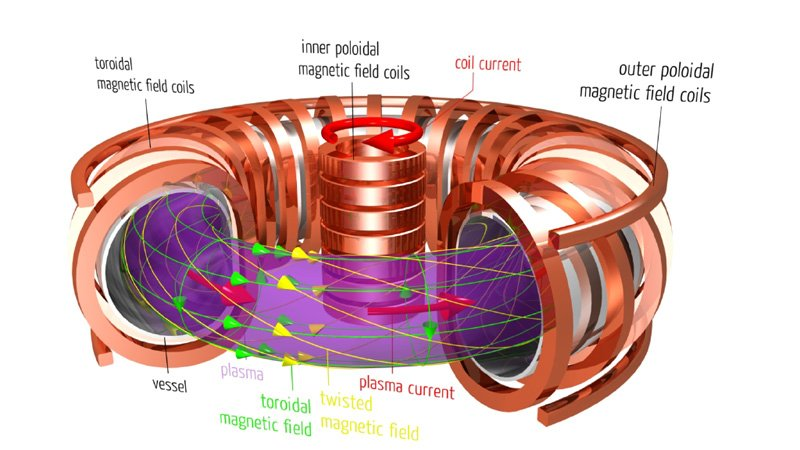
\includegraphics[width=1\textwidth]{Trasformatore/tokamak_scheme.jpg}
	\caption[Schema interno di un Tokamak]{Interno Tokamak}
\end{figure}

\noindent
Le bobine (poloidali e toroidali) servono a controllare il plasma presente nel \textit{Vessel} dell'impianto e confinare il Plasma all'interno di un flusso compresso dentro la camera, le alte temperature e la forte compressione a cui è sottoposto il Plasma, permette di realizzare eventi di \textbf{Fusione Nucleare} tra gli atomi di idrogeno a base del plasma.\\
L'interazione tra le \textbf{Bobine e Plasma}, ha un modello matematico non dissimile da quello di \textbf{Trasformatore Elettrico} nella relazione \textit{Primario-Secondario} (con i dovuti paragoni e le ovvie \nonLinearita presenti nel caso di un impianto Tokamak reale).\\
Grazie a questa similitudine è stato possibile replicare in sicurezza la fisica presente all'interno di un Tokamak, nell'ambiente controllato del laboratorio.\\

\subsection{Richiami di elettronica}
Prima di modellare ed analizzare l'esperimento della tesi, è necessario richiamare qualche proprietà/concetto di elettronica per poter comprendere i passaggi matematici e fisici:
\vspace{-5mm}
\NumTabs{7}
\begin{itemize}[itemsep=-4mm]
	\item \nameref{th:KirchhoffNodi}
	\item \nameref{th:KirchhoffMaglie}
	\item \nameref{def:induttoreIdeale}
	\item \nameref{def:induttanza}
	\item \nameref{def:trasformatoreIdeale}
\end{itemize}


\begin{teorema}[Prima legge di Kirchhoff (legge dei nodi)\label{th:KirchhoffNodi}]
	La somma algebrica delle intensità di corrente nei rami facenti capo allo stesso nodo è nulla.
	\begin{empheq}[box=\mathStep]{equation} \label{eq:KirchhoffNodi}
		\sum I_k = 0
	\end{empheq}
\end{teorema}

\begin{teorema}[Seconda legge di Kirchhoff (legge delle maglie)\label{th:KirchhoffMaglie}]
	La somma algebrica delle f.e.m. agenti lungo i rami di una maglia è uguale alla somma algebrica dei prodotti delle intensità di corrente di ramo per le rispettive resistenze (del ramo).
	\begin{empheq}[box=\mathStep]{equation} \label{eq:KirchhoffMaglie}
		\sum_{\forall k} V_k = \sum_{\forall k} f_{em_k}
	\end{empheq}
\end{teorema}
\vspace{-5mm}
\noindent
Oltre ai teoremi di Kirchhoff, che ci serviranno per ricavare le equazioni della dinamica, enunciamo ora le proprietà degli induttori, indispensabili per poter definire la loro relazione Corrente/Tensione.

\begin{de}[Induttore Ideale\label{def:induttoreIdeale}]
	Un Induttore Ideale si oppone solo alle variazioni di corrente, variando la tensione ai suoi capi di conseguenza, non presenta nessuna resistenza elettrica in caso di correnti costanti ai suoi capi.\\
	Il suo valore è dato dal \textbf{coefficiente di autoinduzione}, tipicamente espresso con il simbolo $L$, la cui unità di è l'Henry [$H$].\\
	Un Induttore accumula energia all'interno di un campo magnetico, e questa relazione è descritta dall'equazione:
	\begin{empheq}[box=\mathStep]{equation} \label{eq:flussoMagnetico}
		\Phi _{B}=Li
	\end{empheq}
	$ \Phi _{B} $ := \textbf{Flusso magnetico}; $L$ := \textbf{Coefficiente di autoinduzione}\\
	Dalla legge di Faraday(ignorando momentaneamente la conservazione dell'energia, ovvero la legge di Lenz), applicata alla circuitazione del circuito costituito dalla induttanza stessa, si ha:
	\begin{empheq}[box=\mathStep]{equation}
		\displaystyle {\frac {d\Phi _{B}}{dt}}=V
	\end{empheq}
	Dove V è il potenziale indotto ai morsetti del circuito in questione. Perciò, derivando l'equazione \ref{eq:flussoMagnetico} ad entrambi i membri rispetto al tempo, si ottiene:
	\begin{empheq}[box=\mathStep]{equation}
		\displaystyle \frac {d\Phi _{B}}{dt}=L{\frac  {di}{dt}}+i{\frac  {dL}{dt}}
	\end{empheq}
	In molti casi fisici, però, l'induttanza può essere considerata costante rispetto al tempo (o tempo-invariante), da cui:
	\begin{empheq}[box=\mathStep]{equation}
		\displaystyle {\frac {d\Phi _{B}}{dt}}=L{\frac {di}{dt}}
	\end{empheq}
	Combinando le equazioni precedenti si ha:
	\begin{empheq}[box=\mathCalc]{equation}
		{\displaystyle V(t)={L{\frac {di(t)}{dt}}}} \Leftrightarrow i(t) = \frac{1}{L} \int V(t) dt
	\end{empheq}
\end{de}

\noindent
Nel calcolo della \ref{eq:flussoMagnetico}, abbiamo omesso la legge di Lenz, poichè per parametrizzare l'induttore il segno "-" complica inutilmente i calcoli essendo assegnato dalla polarizzazione del circuito esaminato.\\
Essa al contrario, prende un importanza notevole in presenza di fenomeni di \textbf{Induttanza}:
\begin{de} [Induttanza\label{def:induttanza}]
	L'induttanza è la proprietà dei circuiti elettrici tale per cui la corrente (intesa variabile nel tempo) che li attraversa induce una \textbf{Forza ElettroMotrice} (f.e.m.) Indotta che si oppone alla variazione di corrente, per la legge di Lenz.
	In questi scenari (vedi Trasformatore Elettrico ad esempio), 2 ciruiti sono accoppiati magneticamente tra di loro attraverso 2 induttori, si ottiene quindi che, la variazione del flusso magnetico da parte del primo induttore, crea una \textbf{Forza ElettroMotrice} (f.e.m.) indotta contraria:
	\begin{empheq}[box=\mathCalc]{equation}
		{\displaystyle -{\frac {d\Phi _{B}}{dt}}={\mathcal {E}}=V}
	\end{empheq}
	Dove $ \mathcal{E} $ è la \textbf{Forza ElettroMotrice} (f.e.m.) indotta.
\end{de}
\noindent
Per finire, unendo insieme i concetti di \nameref{def:induttoreIdeale} e \nameref{def:induttanza} è possibile ottenere la descrizione matematica di un Trasformatore Monofase Ideale (\cite{Transformatore}\footnote{Senso di misura del secondario opposto nell'articolo a quello qui presentato}):
\begin{figure}[h]
	\centering
	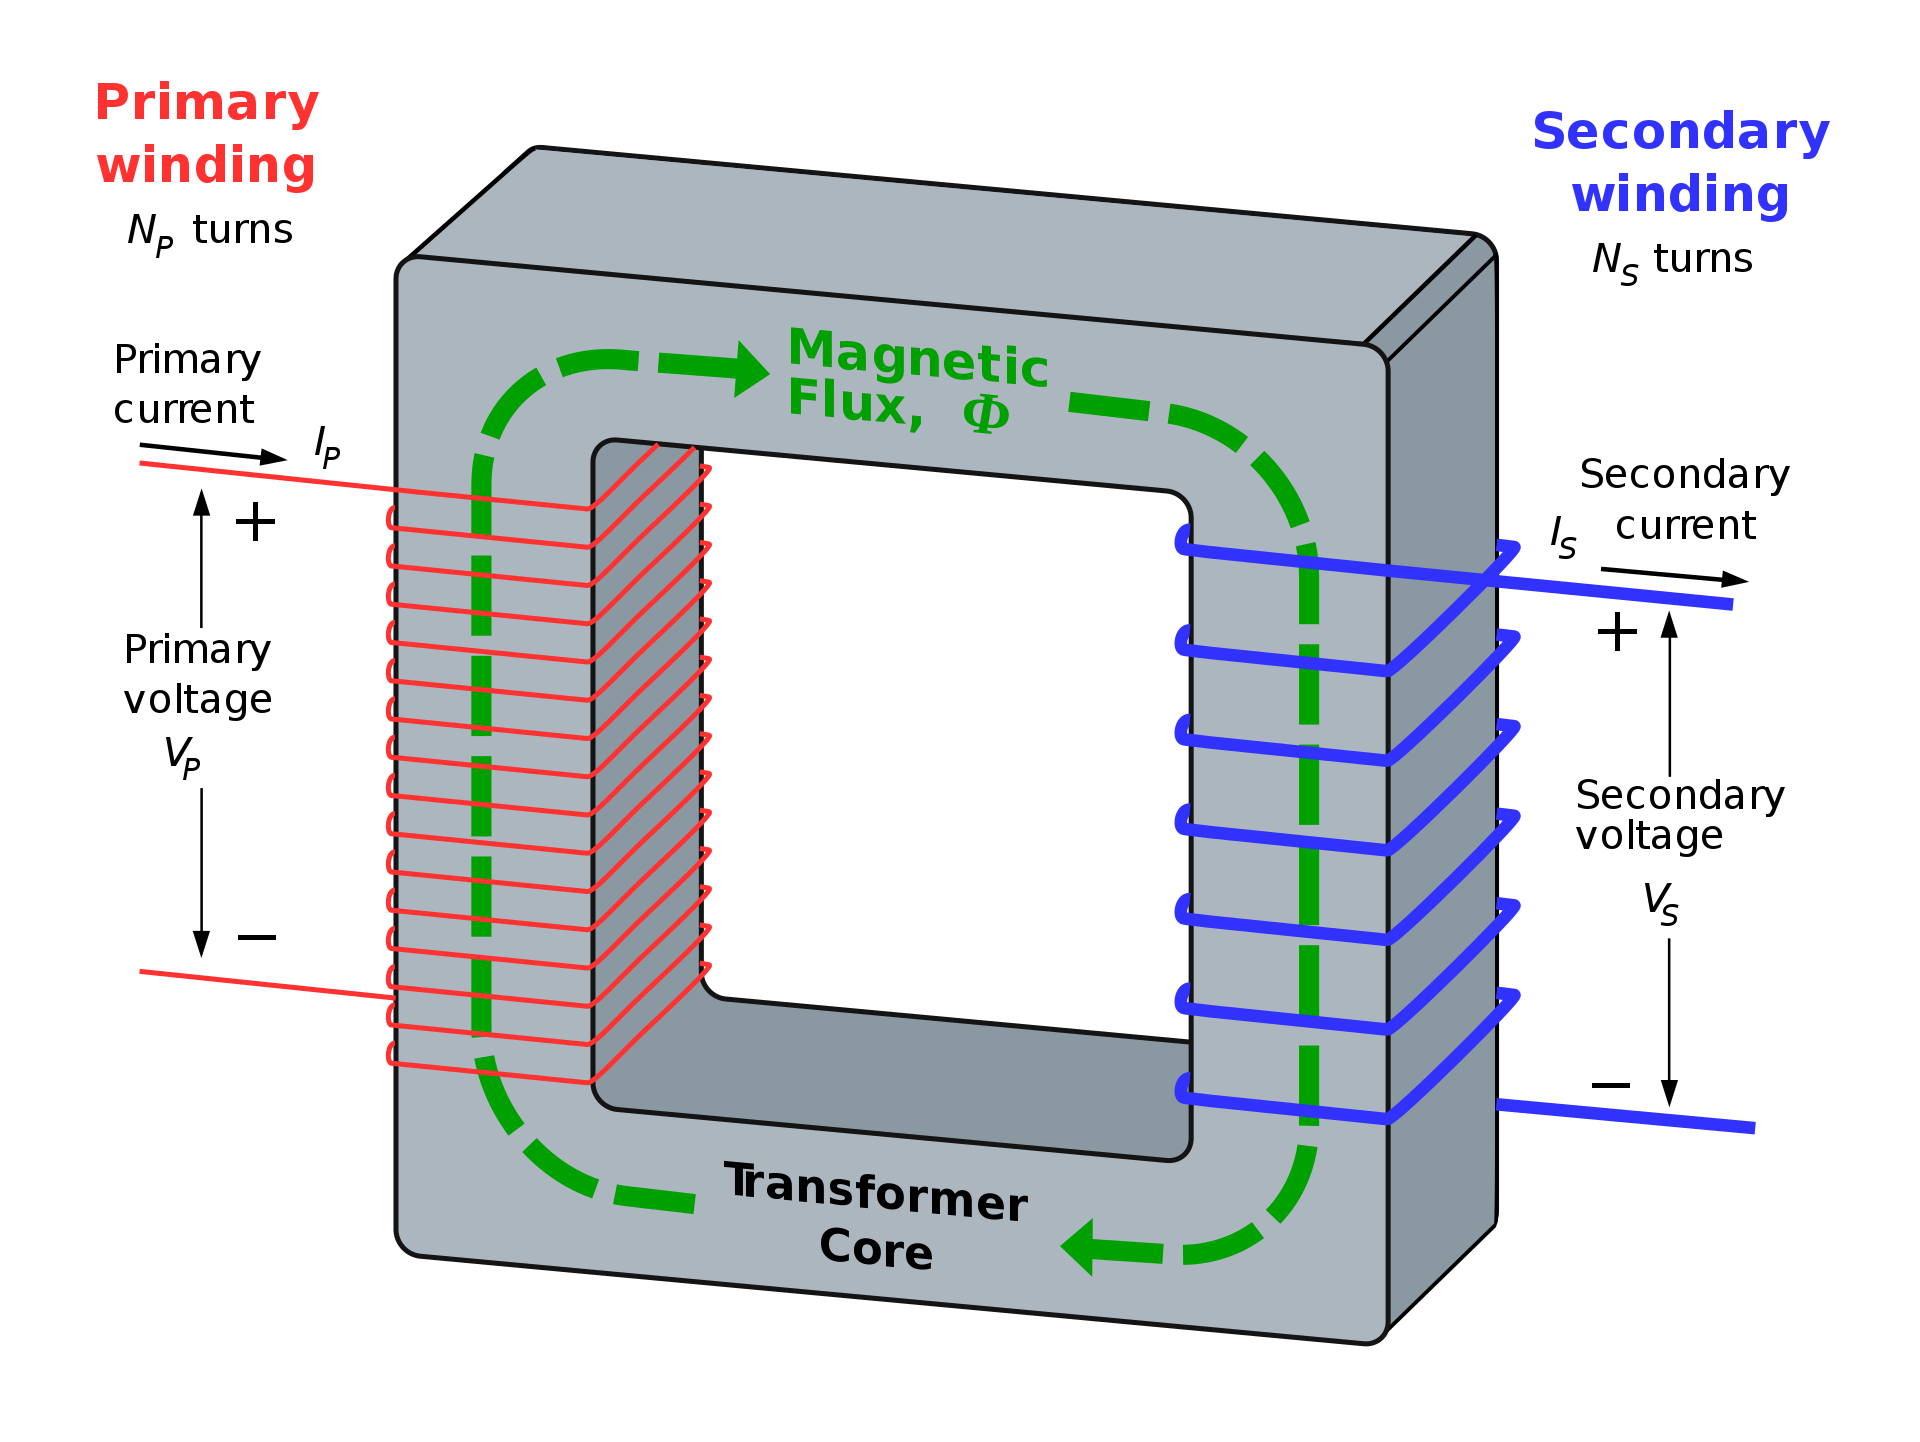
\includegraphics[width=0.8\textwidth]{Trasformatore/trasformatore.png}
	\caption[Trasformatore ideale con Campo magnetico]{Trasformatore Ideale}
\end{figure}

\begin{de}[Trasformatore Ideale Monofase\label{def:trasformatoreIdeale}]
	Il Trasformatore è una macchina elettrica, basata sul fenomeno dell'induzione elettromagnetica, destinata a trasformare, tra il circuito primario (ingresso) e il circuito secondario (uscita) del trasformatore, i fattori tensione e corrente della potenza elettrica.\\
	Trasferisce quindi energia elettrica da un circuito elettrico a un altro che ha una tensione diversa, accoppiandoli induttivamente, senza che siano a contatto tra loro gli avvolgimenti del trasformatore.
	Il trasformatore è una macchina reversibile.\\
	
	Il Trasformatore è costruito affinché il circuito Primario e il Secondario condividano lo stesso campo magnetico, e quindi lo stesso flusso $\Phi _{B}$.\\
	Nel caso ideale, quindi, si ha che:\\
	\begin{empheq}[box=\mathCalc]{equation}
		\Phi_{B} = \Phi_{B_P} - \Phi_{B_S}
	\end{empheq}
	Siccome tale flusso varia nel tempo, induce nei due avvolgimenti le f.e.m.(\nameref{def:induttanza}):
	\begin{empheq}[box=\mathCalc]{equation}
		e_p = N_1 \frac{d \Phi_{B}}{dt} ; e_s = -N_2 \frac{d \Phi_{B}}{dt}
	\end{empheq}
	I segni non sono entrambi concordi a causa del verso del flusso, che nel primario è concorde e nel secondario discorde (e qui torna la forza di Lenz).\\
	Viste dai morsetti del trasformatore, abbiamo che le tensioni istantanee (dovute alle correnti presenti nei 2 rami) sono pari a:
	\begin{empheq}[box=\mathCalc]{equation} \label{eq:tensioneTrasformatore}
		\displaystyle \left \{ \begin{array}{l}
			V_{P} = R_P I_P + L_{PP} \dot I_P - L_{SP} \dot I_S \\
			V_{S} = R_S I_S - L_{PS} \dot I_P + L_{SS} \dot I_S \\
		\end{array}
		\right.
	\end{empheq}
	Dove $R_P$ e $R_S$ rappresentano le resistenze equivalenti viste dai morsetti (i carichi).\\
	Con i coefficienti di mutua induttanza che si ricavano dalla Def di \nameref{def:induttoreIdeale}:
	
	\begin{center}
		\begin{tabular}[t]{c c}
			$ \displaystyle L_{pp} = \frac{N_P  \Phi_{B_P} }{i_P} $ & $ \displaystyle L_{ps} = \frac{N_S  \Phi_{B_P} }{i_P} $ \\[5mm]
			$ \displaystyle L_{sp} = \frac{N_P  \Phi_{B_S} }{i_S} $ & $ \displaystyle L_{ps} = \frac{N_S  \Phi_{B_S} }{i_S} $
		\end{tabular}
	\end{center}
\end{de}

\noindent
Arrivati a questo punto abbiamo gli strumenti necessari per poter modellare matematicamente l'esperimento.
\newpage

\subsection{Modellazione Fisica}
%La fisica che descrive la dinamica di un Plasma passa per la soluzione della \textbf{Equazioni alle derivate parziali di Grad-Shafranov} (\textit{Grad-Shafranov PDE}).
Usando i concetti esposti, vediamo ora una buona approssimazione con modello lineare della dinamica tra \textbf{Bobina e Plasma}.\\
Come descritto nell'articolo di \cite{TokamakCircuit}, è possibile modellare la dinamica \textbf{Bobina - Plasma} come fosse il circuito di un
\nameref{def:trasformatoreIdeale}:
\begin{figure}[h]
	\centering
	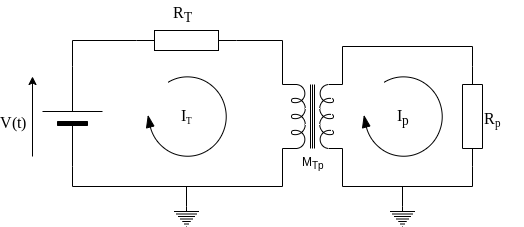
\includegraphics[width=1\textwidth]{Trasformatore/PlasmaCircuit-PlasmaCircuit.png}
	\caption[Circuito Equivalente Bobina/Plasma all'interno di un Tokamak]{Circuito Equivalente Bobina/Plasma}
\end{figure}
\NumTabs{11}
\begin{leg}
	\item $V(t)$\tab:= Tensione di controllo della Corrente $I_T$
	\item $I_T$\tab:= Corrente del Trasformatore
	\item $R_T$\tab:= Resistenza equivalente Trasformatore
	\item $I_p$\tab:= Corrente di Plasma
	\item $R_p$\tab:= Resistenza di Plasma
	\item $M_{Tp}$\tab:= Coefficiente di Induttanza Trasformatore $\rightarrow$ Plasma
\end{leg}
\paragraph{Difformità dalla realtà} Nella realtà $R_p$ e $M_{Tp}$ sono dei parametri che variano in funzione dello stato del plasma (Temperatura, Energia, Evoluzione dell'esperimento, ecc\ldots), ma per ovvie ragioni di difficoltà nel riprodurre in laboratorio simili \nonLinearita, noi prenderemo per costanti questi parametri.

\subsection{Semplificazione Primario - Secondario}
Sempre dallo stesso articolo di \cite{TokamakCircuit}, si evince che è possibile modellare questa relazione tra i 2 circuiti prendendo in considerazione \textbf{solo} le forze di induzione dovute alla corrente che il Primario trasferisce sul Secondario, ciò permette di semplificare ulteriormente il circuito trascurando le correnti indotte dal Plasma dentro la Bobina del Primario.\\
Usando queste osservazioni si ottiene quindi il circuito equivalente:
\begin{figure}[h]	\label{fig:PlasmaSemplificato}
	\centering
	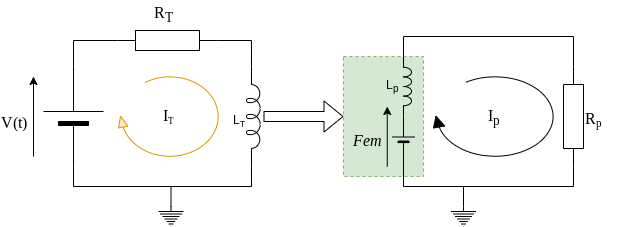
\includegraphics[width=1\textwidth]{Trasformatore/PlasmaCircuit-EquivalentCalc.png}
	\caption[Circuito Equivalente Bobina/Plasma all'interno di un Tokamak trascurando l'induzione del plasma verso la bobina]{Circuito equivalente Bobina/Plasma semplificato}
	
\end{figure}

\NumTabs{11}
\begin{leg}
	\item $V(t)$\tab:= Tensione di controllo della corrente $I_T$
	\item $I_T$\tab:= Corrente del Trasformatore
	\item $R_T$\tab:= Resistenza equivalente Trasformatore
	\item $I_p$\tab:= Corrente di Plasma
	\item $R_p$\tab:= Resistenza di Plasma
	\item $M_{Tp}$\tab:= Coefficiente di Induttanza Trasformatore $\rightarrow$ Plasma
	\begin{itemize} [topsep=-1mm,itemsep=0mm]
		\item $L_T$\tab:= Induttanza equivalente Trasformatore
		\item $L_p$\tab:= Induttanza equivalente Plasma
	\end{itemize}
\end{leg}
\noindent
Usando questa semplificazione dall'equazione \ref{eq:tensioneTrasformatore} del trasformatore ignoriamo che la tensione sul Primario è influenzata dal Secondario; in questa condizione il circuito del Primario evolve come sistema indipendente rispetto al Secondario, e la sua evoluzione influenza il Secondario.

\newpage
\subsection{Dal circuito alla dinamica}\label{subsec:dinamicaCircuito}
Analizziamo ora la dinamica del circuito \ref{fig:PlasmaSemplificato}.
\subsubsection{Dinamica di Plasma}
\vspace{-5mm}
Iniziando dal calcolare la dinamica nella corrente di Plasma usando la \nameref{th:KirchhoffMaglie}:
\begin{empheq}[box=\mathStep]{equation*}
	F_{em} = L_p \dot I_p + I_p R_p
\end{empheq}
Sappiamo in oltre che la $F_{em}$, grazie all'\nameref{def:induttanza} del circuito è pari a: 
\begin{empheq}[box=\mathStep]{equation*}
	F_{em} = -M_{Tp} \dot I_T
\end{empheq}
Da cui otteniamo:
\begin{empheq}[box=\mathCalc]{equation} \label{eq:correntePlasmaDinamica}
	-M_{Tp} \dot I_T = L_p \dot I_p + I_p R_p
\end{empheq}
{\footnotesize Da notare la somiglianza con l'equazione del trasformatore \ref{eq:tensioneTrasformatore}}.\\
Dalla eq \ref{eq:correntePlasmaDinamica} possiamo notare che rendere la corrente di Plasma costante, equivale a fissare una $F_{em}$ di riferimento costante, ed essendo problematico misurare la corrente direttamente nel plasma reale, usiamo la \textbf{Tensione di Loop}, che nel caso del trasformatore equivale alla tensione di uscita del Trasformatore.

\subsubsection{Dinamica del Trasformatore}
\vspace{-5mm}
Vediamo ora la dinamica della corrente del Trasformatore, in funzione della \textit{Tensione di controllo}:\\
Sempre grazie alla \nameref{th:KirchhoffMaglie} scriviamo:
\begin{empheq}[box=\mathCalc]{equation} \label{eq:correnteTrasformatoreDinamica}
	V(t) = L_T \dot I_T + I_T R_T
\end{empheq}

\subsection{Funzione di Trasferimento}
Nella sezione \ref{subsec:dinamicaCircuito} abbiamo ottenuto la dinamica istantanea dei 2 rami del circuito \ref{fig:PlasmaSemplificato}, ricaveremo ora le funzioni di trasferimento dei 2 rami e troveremo la dinamica del Trasformatore.
\subsubsection{Funzione di Trasferimento Plasma}
\vspace{-5mm}
Partendo dall'equazione \ref{eq:correntePlasmaDinamica}, supponendo condizioni iniziali nulle, abbiamo:
\begin{empheq}[box=\mathStep]{equation*}
	s I_p L_p  + I_p R_p = -s I_T M_{Tp} \Rightarrow I_p( s L_p + R_p) = -s I_T M_{Tp} \Rightarrow I_p(s) = \frac{-s M_{Tp}}{( s L_p + R_p)} I_T(s)
\end{empheq}
La cui, funzione di trasferimento risulta essere:
\begin{empheq}[box=\mathCalc]{equation} \label{eq:correntePlasmaLaplace}
	\frac{I_p(s)}{I_T(s)}  = \frac{-s M_{Tp}}{( s L_p + R_p)}
\end{empheq}

\subsubsection{Funzione di Trasferimento Trasformatore}
\vspace{-5mm}
Similmente, partendo dall'equazione \ref{eq:correnteTrasformatoreDinamica} si ricava:
\begin{empheq}[box=\mathStep]{equation*}
	s I_T L_T  + I_T R_T = V(s) \Rightarrow I_T( s L_T + R_T) = V(s) \Rightarrow I_T(s) = \frac{1}{(s L_T + R_T)} V(s)
\end{empheq}

La cui, funzione di trasferimento risulta essere:
\begin{empheq}[box=\mathCalc]{equation} \label{eq:correnteTrasformatoreLaplace}
	\frac{I_T(s)}{V(s)}  = \frac{1}{(s L_T + R_T)}
\end{empheq}

\begin{oss} \label{oss:Iref}
	La funzione di trasferimento che abbiamo ottenuto rispecchia il circuito dell'esperimento, noi però abbiamo un sistema che si controlla in corrente e che ha un uscita in corrente potremmo allora riassegnare l'ingresso come:
	\begin{empheq}[box=\mathCalc]{equation*}
		V(t)=I_{ref}(t) \cdot R_T \Rightarrow I_{ref}(t) = \frac{V(t)}{R_T}
	\end{empheq}
	Ottenendo così: 
	\begin{empheq}[box=\mathStep]{equation}
		I_T(s) = \frac{R_T}{(s L_T + R_T)} I_{ref}(s) = \frac{1}{(s \frac{L_T}{R_T} + 1)} I_{ref}(t)
	\end{empheq}
	In questa forma possiamo osservare che, per $I_{ref}(t)=I_{ref}$ costante, superato il transitorio, si ottiene $I_T = I_{ref}$, da cui abbiamo che la corrente sul trasformatore viene attuata con un certo ritardo dovuto alla costante di tempo $\tau = \frac{L_T}{R_T}$
\end{oss}

\subsubsection{Funzione di Trasferimento Complessiva}\label{subsubsec:FuncTrasfImpianto}
\vspace{-5mm}
Connettendo in serie i 2 blocchi e tenendo conto dell'osservazione \ref{oss:Iref} si ottiene:
%\vspace{-3mm}
\begin{empheq}[box=\mathCalc]{equation} \label{eq:FuncTrasfTot}
	P(s) = \frac{I_p(s)}{I_{ref}(s)} = \frac{I_T(s)}{I_{ref}(s)} \cdot \frac{I_p(s)}{I_T(s)}  = -\frac{s M_{Tp}}{( s L_p + R_p)(s L_T + R_T)}
\end{empheq}

\noindent
Che vista come schema a blocchi diventa:
\begin{figure}[h]
	\centering
	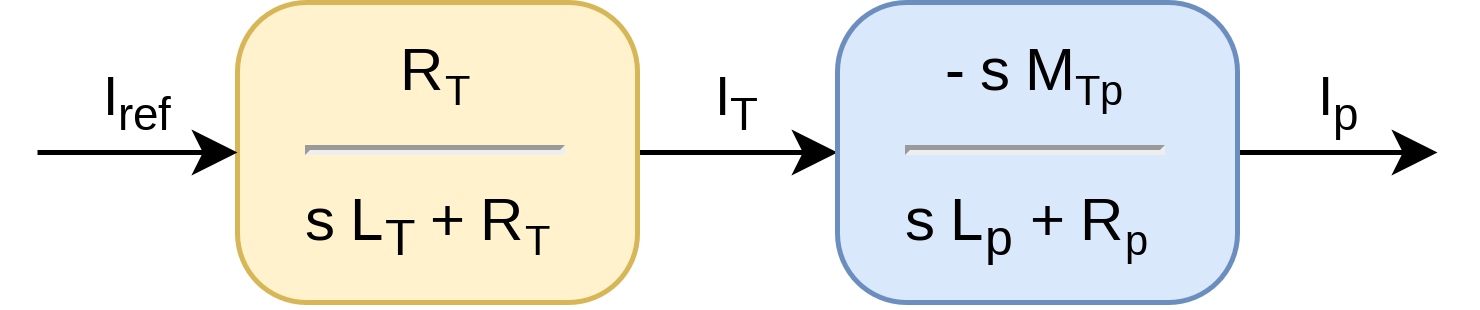
\includegraphics[width=1\textwidth]{Trasformatore/PlasmaCircuit-SchemaBlocchi.png}
	\caption[Schema a Blocchi della funzione di trasferimento della corrente di Plasma]{Schema a Blocchi Corrente di Plasma}
\end{figure}

\noindent
Essendo in uscita il segno delle correnti inverso dall'ingresso, possiamo eliminare questo fastidioso problema di segno in molti modi, quello che si è usato da qui in avanti nella realizzazione della tesi e degli esperimenti, è stato banalmente invertire i poli del Secondario del trasformatore, ottenendo quindi come funzione di trasferimento:

\begin{empheq}[box=\mathCalc]{equation} \label{eq:FuncTrasfTotPos}
	P_{pos}(s) = -P(s) = \frac{s M_{Tp}}{( s L_p + R_p)(s L_T + R_T)} = \frac{-I_p(s)}{I_{ref}(s)}
\end{empheq}
\newpage


\section{Trasduttore di Corrente}\label{CurrentSense}
Come detto nell'introduzione, l'obiettivo della tesi è di controllare la corrente sul secondario usando il campo elettrico del secondario, la misura della corrente scorrente sul primario in tale ottica non sarebbe una misura di interesse. Essendo però un lavoro di ricerca, si è preferito poter misurare la corrente effettivamente circolante nel Primario del trasformatore, così da poter meglio interpretare i dati di misura senza ambiguità.\\
\begin{figure}[h]
	\centering
	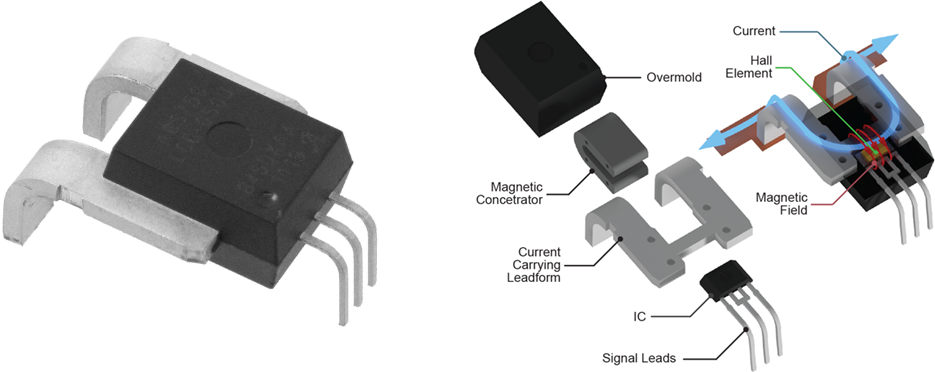
\includegraphics[width=1\textwidth]{ACS770/ACS770-Fig.png}
	\caption[Sensore di Corrente \citefield{ACS770}{series}]{Sensore di Corrente}
\end{figure}
%\vspace{-1cm}
\subsection{Sensore scelto}
Per misurare la corrente del primario, si è posizionato in serie allo stesso il sensore di Corrente \cite{ACS770}.\\
La famiglia di sensori ha in generale le seguenti caratteristiche: \vspace{-5mm}
\begin{center}
	\begin{tabular}[t]{|l r|}
		\hline
		Bandwidth:                             & 120 kHz                               \\
		Output rise time :                     & 4.1 $ \mu s $                         \\
		Ultralow power loss:                   & 100 $ \mu \Omega $ Resistenza Interna \\
		Single supply operation                & 4.5 to 5.5 V                          \\
		Extremely stable output offset voltage &                                       \\
		\hline
	\end{tabular}
\end{center}

\noindent
In oltre, delle tante varianti presenti, si è scelto di usare la \citefield{ACS770}{series}, le cui caratteristiche chiave sono:

\begin{center}
	\begin{tabular}[t]{|l r|}
		\hline
		Primary Sampled Current: & $\pm$ 100 A     \\
		Sensitivity Sens (Typ.)  & 20(mV/A)        \\
		Current Directionality   & Bidirectional   \\
		$T_{OP}$                 & –40 to 150 (°C) \\
		\hline
	\end{tabular}
\end{center}

\noindent
L'ampio margine di misura, e la robustezza alle variazioni di temperatura rendono rendono il dispositivo perfetto per misurare i nostri esperimenti.\\
L'ampio margine di misura permette di comprendere tutti i possibili valori di corrente ottenibili in laboratorio, rendendo il prototipo adatto a scopi futuri.\\
\vspace{-8mm}

\subsection{Criticità}
Unico punto dolente è il suo principio di funzionamento: essendo il sensore basato su un l'effetto Hall, ovvero una misura diretta del campo magnetico indotto dalla corrente nel conduttore, è importante tenere distante il sensore dal Trasformatore Centrale che nei suoi momenti di massimo flusso di corrente, genera ovviamente un campo magnetico non indifferente.

\subsection{Funzionamento Interno}
\vspace{-5mm}
\begin{figure}[h]
	\centering
	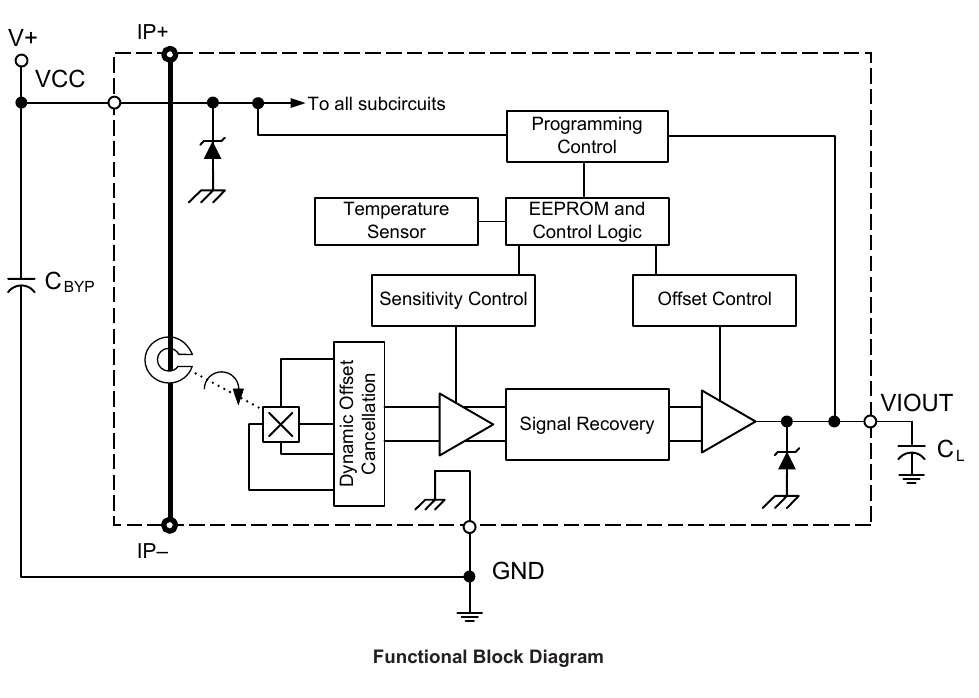
\includegraphics[width=0.8\textwidth]{ACS770/ACS770-SchemaBlocchi.png}
	\caption[\citefield{ACS770}{series} Schema a Blocchi]{Schema a Blocchi}
\end{figure}
\noindent
Tra le caratteristiche chiave dell'\cite{ACS770}, troviamo il disaccoppiamento fisico tra la corrente da misurare e il circuito di misura.\\
Questa caratteristica chiave, garantisce la salvaguardia del circuito logico a valle, dai possibili eventi catastrofici a monte.\\
Esso è in oltre fornito di sensori di temperatura e sistemi di \textit{Signal Recovery} che permettono all'Hardware stesso di compensare parzialmente \nonLinearita termiche e nella misura dell'effetto Hall, ottenendo un output assimilabile a un segnale lineare:

\begin{figure}[h]
	\centering
	\includegraphics[width=1\textwidth]{ACS770/ACS770-Sensibilità.png}
	\caption[\citefield{ACS770}{series} Sensibilità rispetto Temperatura]{Sensibilità}
\end{figure}

\noindent
Come si può vedere dal grafico, gli errori sono tanto più marcati quanto maggiore è la corrente da misurare, ma leggendo dal datasheet abbiamo che questo errore, che dipende si fortemente dalle temperature di esercizio dell'esperimento, non è mai, neanche negli esperimenti più sfortunati, superiore al $\pm2\%$.\\
Anzi, alle temperature $\approx$ 25°, si mantiene contenuto tra $\pm0.5\%$.

\begin{figure}[h]
	\centering
	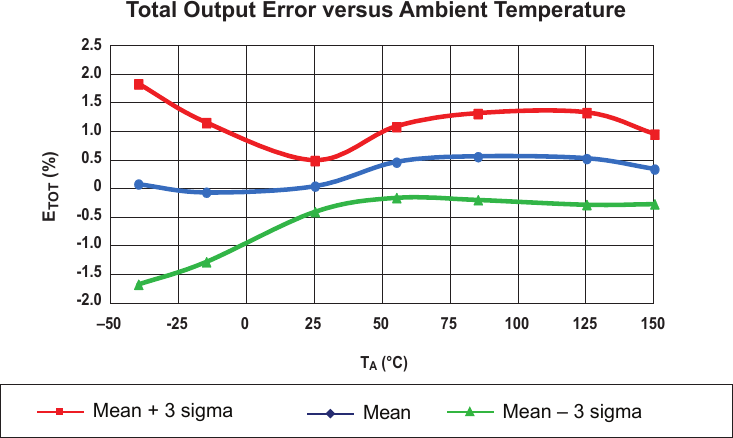
\includegraphics[width=1\textwidth]{ACS770/ACS770-NonLin.png}
	\caption[\citefield{ACS770}{series} \nonLinearita]{Temperatura/NonLinearità}
\end{figure}

\newpage

\subsection{Connessione elettrica}

La connessione del sensore è particolarmente semplice, richiedendo esternamente solo un alimentazione stabilizzata e portando subito in uscita la misura.
\begin{figure}[h]
	\centering
	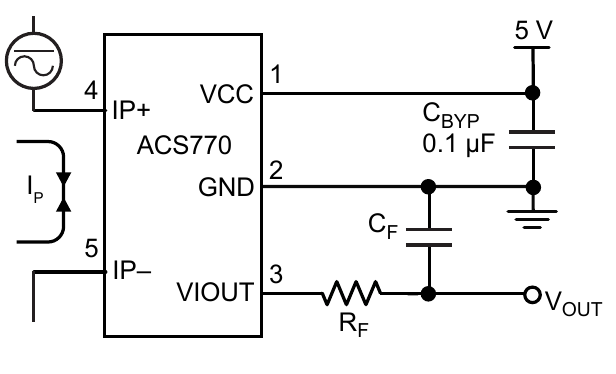
\includegraphics[width=1\textwidth]{ACS770/ACS770-Schema.png}
	\caption[\citefield{ACS770}{series} Schema di collegamento dal Datasheet]{Collegamento dal Datasheet}
\end{figure}

\noindent
Rispetto allo schema proposto dal datasheet, però, si è anche deciso di omettere il filtro passa-basso sulla \textbf{VIOUT}, questa scelta è stata presa per minimizzare il più possibile ritardi di misura della corrente istantanea, poiché le dinamiche del sistema sul secondario, come visto, sono di tipo derivativo, e quindi estremamente rapide.\\

\subsection{Misura}
Il transduttore, misura della corrente sotto forma di tensione, la quale varia in base alla \textbf{Sensibilità} del modello in uso. 
Avendo noi il \citefield{ACS770}{series}, il datasheet riporta:
\begin{center}
	\begin{tabular}[t]{|l r|}
		\hline
		Primary Sampled Current: & $\pm$ 100 A   \\
		Sensitivity Sens (Typ.)  & 20(mV/A)      \\
		Current Directionality   & Bidirectional \\
		\hline
	\end{tabular}
\end{center}

\noindent
Ciò implica che la corrente misurata, è calcolabile come:\\
{\large \begin{center}
	$I_{read} = \frac{V_{Read}[V]}{V_{sense}[V/A]}$
\end{center}
}

\paragraph{Rimozione Offset}
Essendo però il device ad alimentazione singola (0--5V), ma la corrente misurabile Bi-direzionale, sorge la necessità di spostare gli 0A a una tensione superiore agli 0V.\\
Il datasheet riporta che $V_{offset} = \frac{Vcc}{2}\approx$ 2.5V. Da cui deriva che la vera misura di corrente è:
{\LARGE
\begin{empheq}[box=\mathCalc]{equation} \label{eq:Iread}
	I_{read} = \frac{V_{Read}-V_{offset}}{V_{sense}} \frac{V}{[V/A]}
\end{empheq}
}

Al fine di poter misurare l'offset effettivo, durante il set-up viene eseguito a esperimento fermo una misura dell'offset attuale, usando la \nameref{lst:offsetCalc}.\\
Il risultato della computazione, oltre ad essere usato nel controllo è inviato al computer per la post elaborazione dei dati nei grafici.

\paragraph{Analisi Sensibilità}
Usando nell'esperimento un ADC a 10Bit con tensione di riferimento a 5V, abbiamo che la massima sensibilità del \microC, ovvero il suo bit meno significativo è pari a:
%\vspace{-5mm}
\begin{empheq}[box=\mathResult]{equation*}
	V_{step}=\frac{Vcc}{2^{10}-1} = 4,887mV
\end{empheq}
\noindent
Il che equivale a una \textbf{Sensibilità di Corrente} del $\mu$Controllore pari a:
%\vspace{-5mm}
\begin{empheq}[box=\mathResult]{equation*}
	I_{step} =\frac{ V_{step}}{V_{sense}} = 244,379 mA
\end{empheq}
\noindent
Il ché rende la misura buona per osservare cosa stia accadendo, ma sicuramente non sufficientemente densa da poterla usare come parametro ingresso di controllo.

\newpage

\section{Driver di Corrente - IBT-2}\label{CurrentDriver}
Per l'attuazione del controllo di corrente nella bobina primaria del trasformatore, è stato usato il driver di corrente \cite{IBT-2} .


\begin{figure}[h]
	\centering
	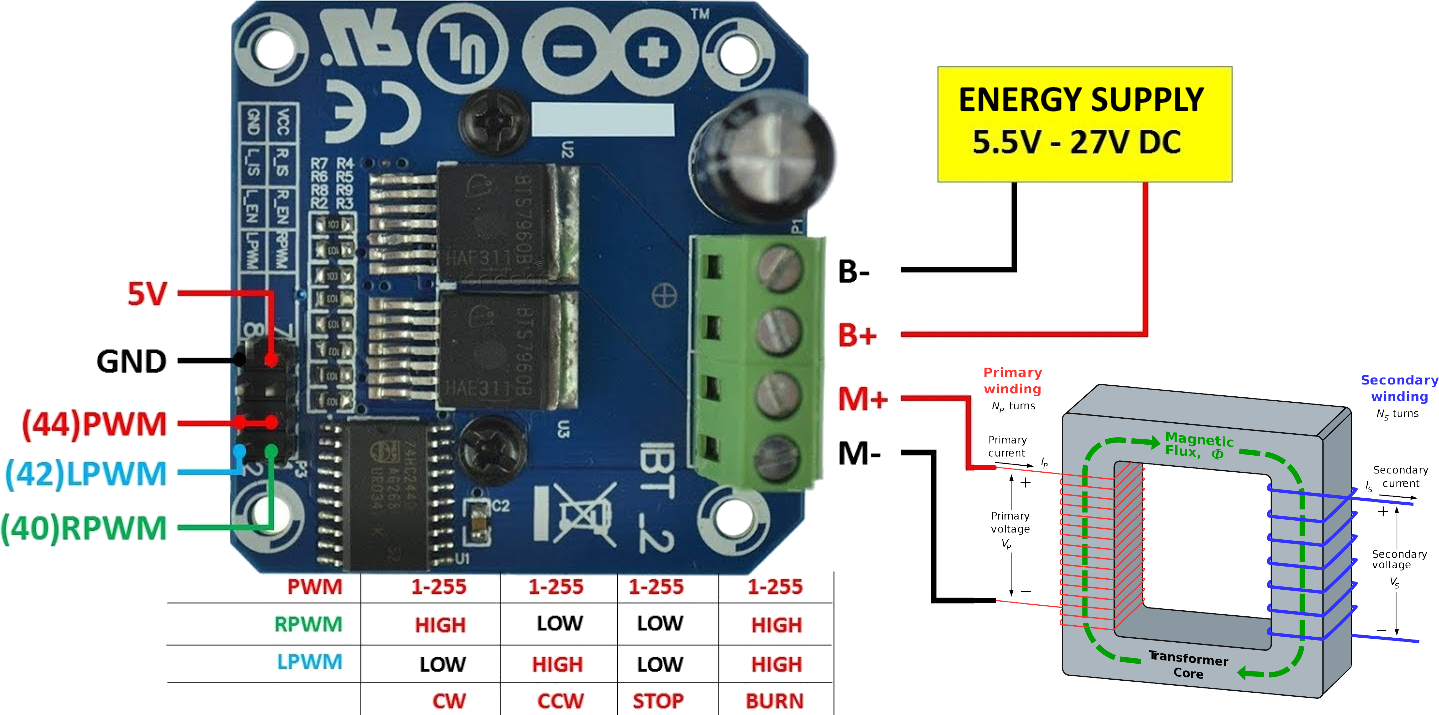
\includegraphics[width=1\textwidth]{IBT-2/TopView.png}
	\caption[Driver Motori IBT-2 TopView \& PinOut]{IBT-2 TopView.}
\end{figure}

\noindent
Esso non è un comune Ponte-H integrato: per poter gestire potenze superiori è stato costruito usando 2 Half-Bridge (\cite{BTS7960b}) collegati assieme mediante una opportuna logica per ricreare un normale Ponte-H.\\
Questa scheda in particola ha prestazioni interessanti per gli scopi di questa tesi, i principali sono elencati di seguito:\vspace{-8mm}
\begin{center}
	\begin{tabular}[t]{|l r|}
		\hline
		Power Input Voltage:                                     & 6 -- 27 V \\
		Peak current:                                            & 43 A      \\
		Massima Frequenza di PWM:                                & 25 kHz    \\
		Protezione Sovra Tensioni                                &           \\
		Disaccoppiamento Ingresso di Potenza/Logica di controllo &           \\
		\hline
	\end{tabular}
\end{center}
\noindent
Di particolare interesse per l'esperimento è proprio la corrente di picco gestibile:
avendo le dinamiche del sistema tempi inferiori ai 5 secondi, poter reggere correnti di picco così elevate rende
la scheda perfetta per i nostri scopi.

\newpage
\subsection{Schema Elettrico}
Al suo interno il driver è composto da 2 Half-Bridge \cite{BTS7960b}, connesse secondo lo schema:
\begin{figure}[h]
	\centering
	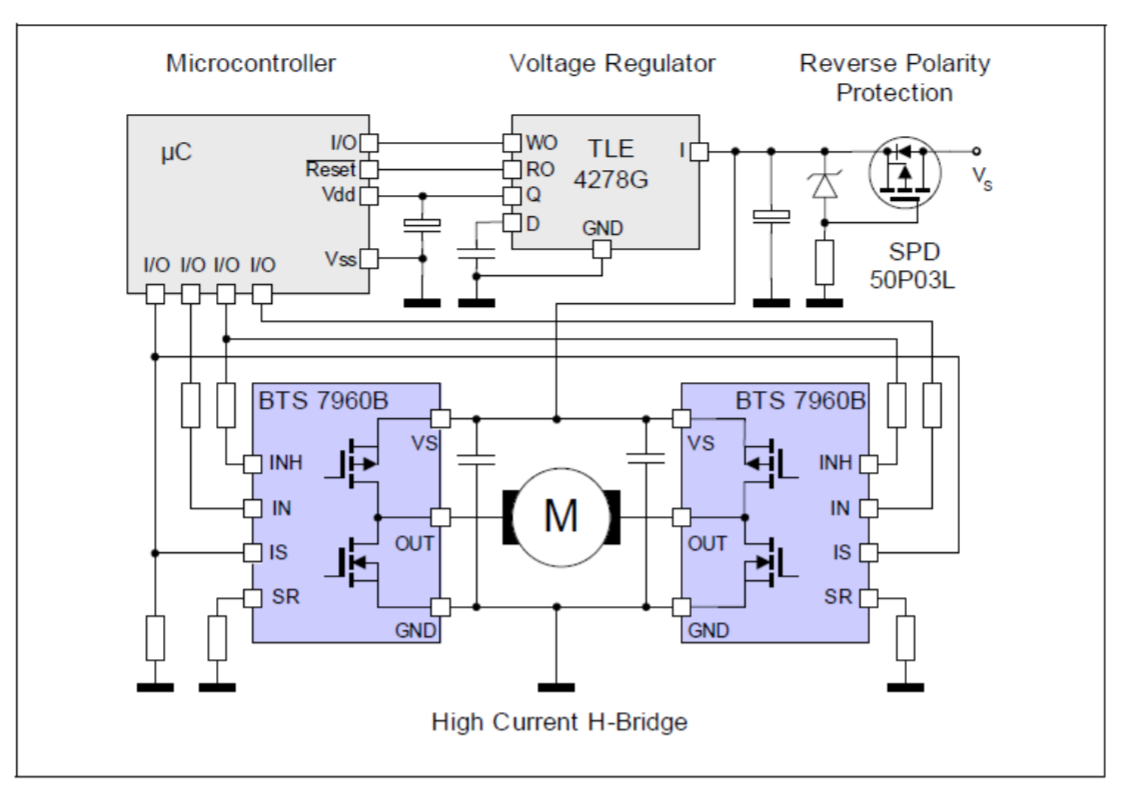
\includegraphics[height=0.5\textheight]{IBT-2/elettricScheme.png}
	\caption[IBT-2 Schema Elettrico]{IBT-2 Schema Elettrico}
\end{figure}\vspace{-5mm}

\noindent
Il \microC è protetto dal carico connesso all'interno del \citefield{BTS7960b}{series}, lasciando al \microC solo il compito di controllare i segnali.


\subsection{Connessione di Controllo}
Il driver permette 2 modalità di funzionamento:
\begin{description}
	\item[Doppio PWM] Modalità operativa che richiede l'uso di 2 PWM\\
	      Ciascun PWM controlla uno dei 2 Half-Bridge, e per evitare di bruciare i driver devono essere controllati singolarmente, il vantaggio di questa configurazione è la possibilità di usare 2 frequenze di controllo diverse.
	\item[Singolo PWM] Modalità operativa classica di un normale Ponte-H\\
	      In questa modalità, la porta nand presente sulla scheda attua la logica di controllo opportuna per governare i 2 Half-Brige come fossero un normale Ponte-H.
\end{description}

\noindent
Per il nostro esperimento si è scelto di usare il collegamento \textbf{\underline{Singolo PWM}} così da evitare spiacevoli sorprese e avere il PWM di controllo sempre sincronizzato.	

\newpage
\subsection{Benchmark del Driver}
Il driver sulla carta à buone prestazioni, ma non sono descritte le sue \nonLinearita, per farle risaltare si sono effettuati 2 esperimenti usando differenti input di controllo:
\begin{enumerate}
	\item \nameref{lst:ondaTriangloare} \\ \vspace{-11mm}
	      \begin{figure}[h]
		      
		      \centering
		      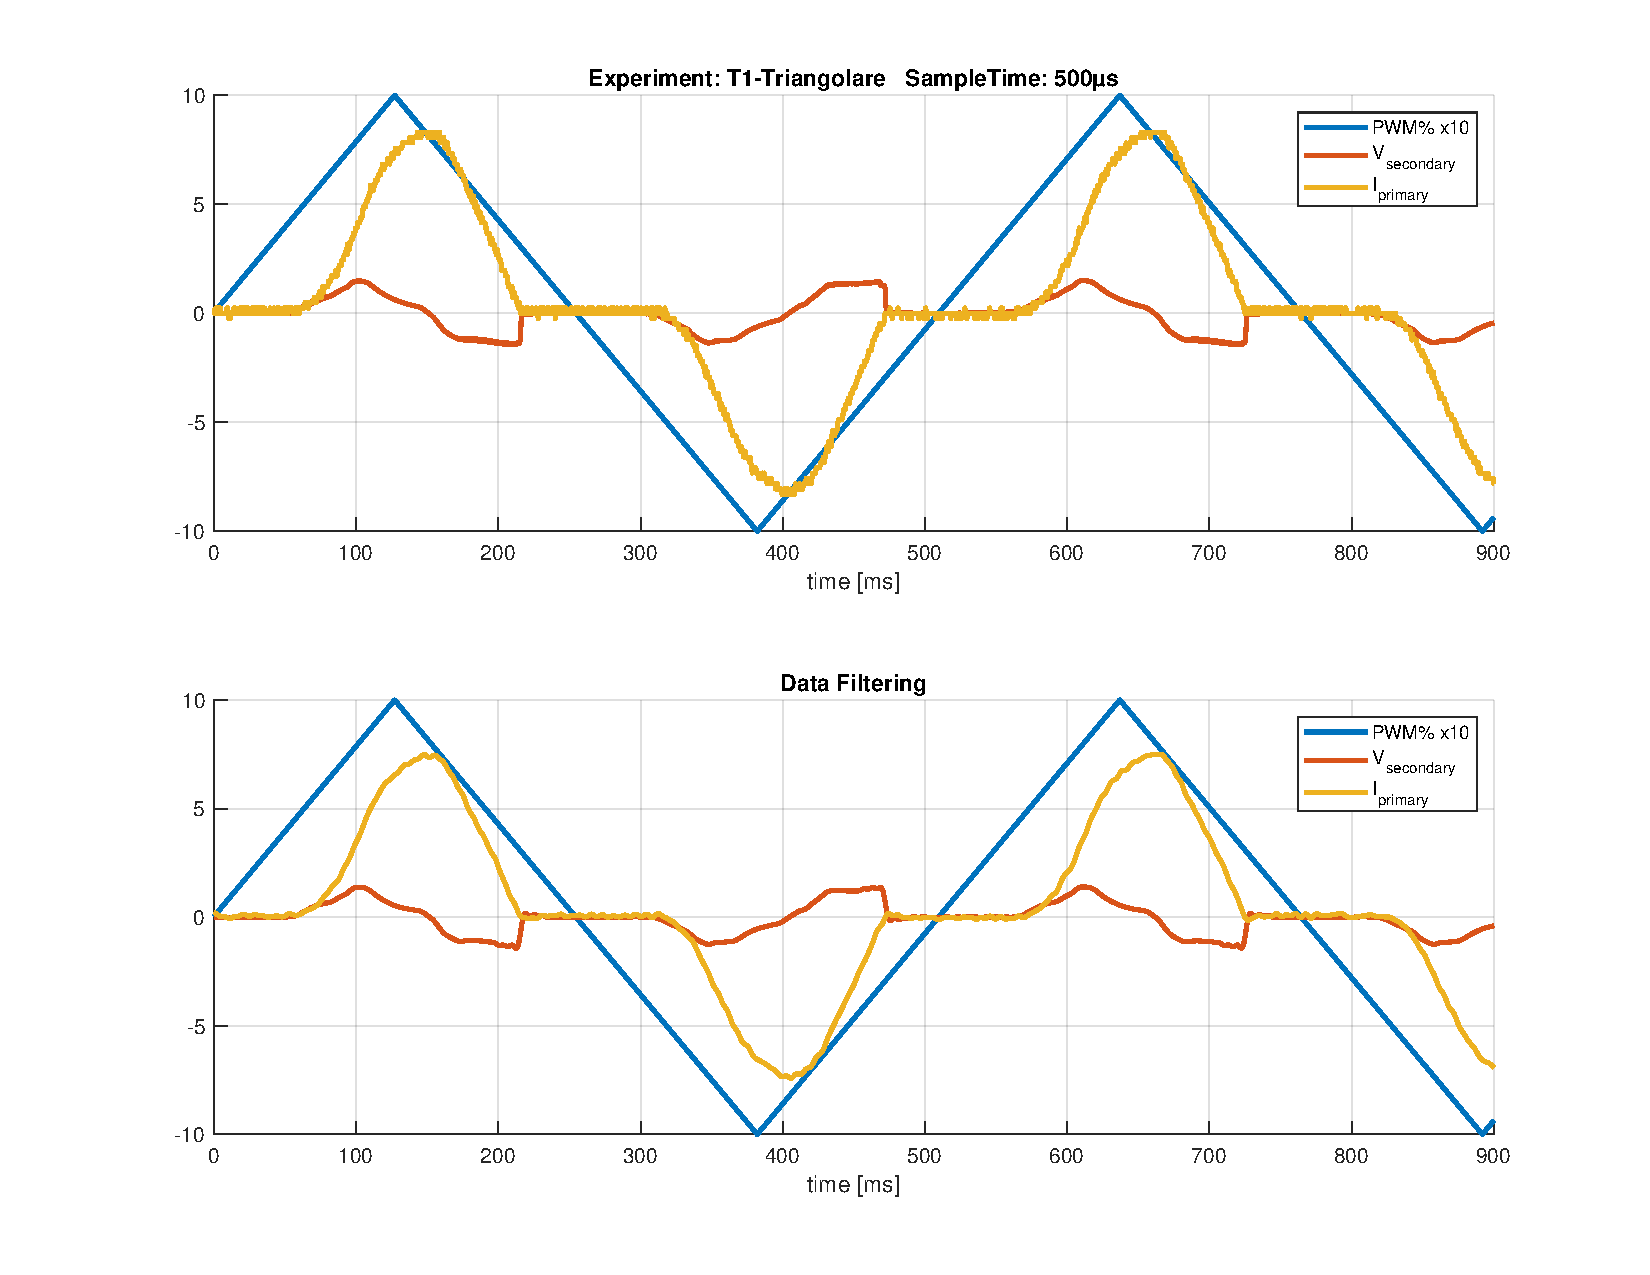
\includegraphics[height=0.5\textheight]{IBT-2/T1-Triangolare.pdf}
		      \caption[Esperimento con Onda Triangolare]{Onda Triangolare}
	      \end{figure}\vspace{-10mm}
	      \paragraph{Dead-Zone Inferiore} L'onda triangolare si presta bene per far risaltare la problematica della Dead-Zone Inferiore, infatti in tutti gli intorni in cui il segnale passa per 0, è possibile vedere come la corrente non vari minimamente, è però possibile notare che i 2 lati non sono simmetrici tra di loro, questo è facilmente spiegabile dal fatto che il primo ha una condizione iniziale $ \neq $ 0 e di fatto stiamo ancora osservando l'esaurimento del transitorio, la soglia di Dead-Zone Inferiore è quindi calcolata vedendo il primo valore di PWM  per cui il sistema risponde a destra degli 0.      
	      
	      \newpage
	\item \nameref{lst:ondaTrapezoidale} \\
	      \begin{figure}[h]
		      \centering
		      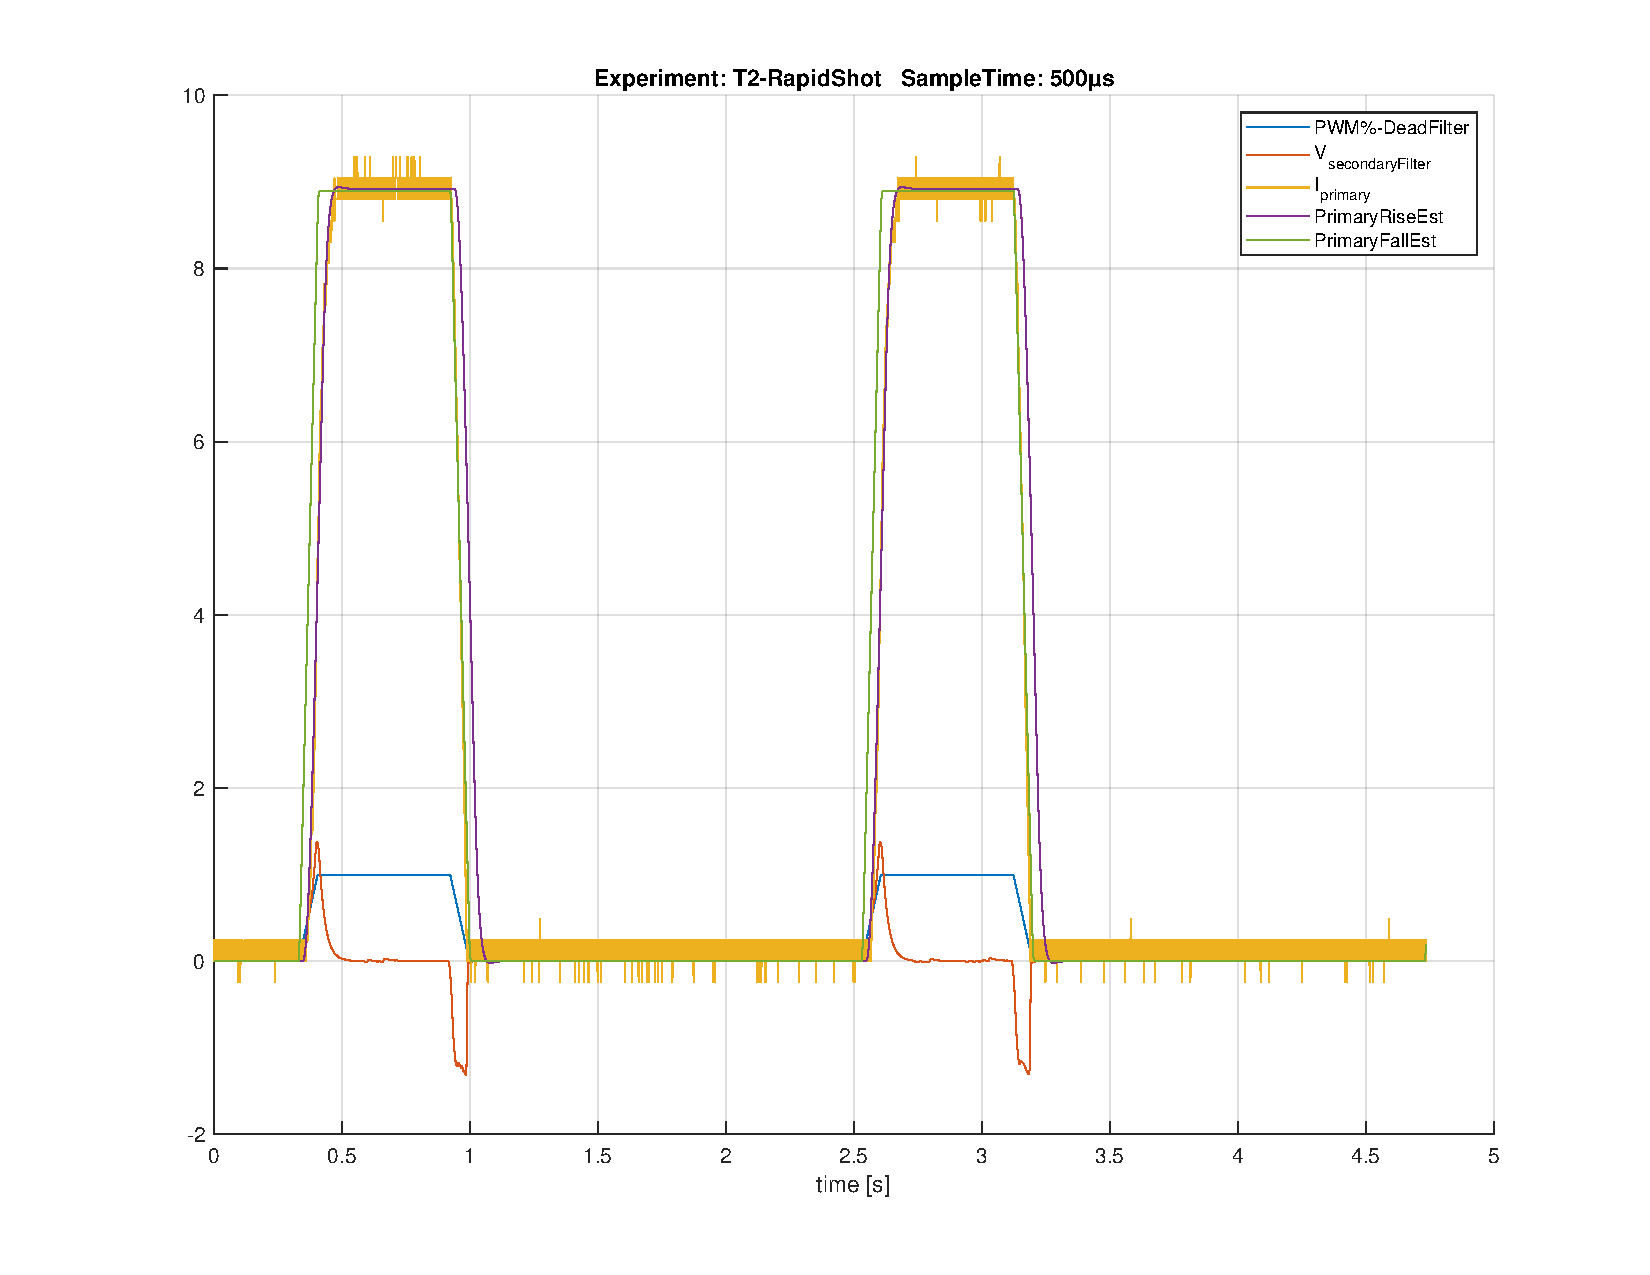
\includegraphics[height=0.5\textheight]{IBT-2/T2-RapidShot.pdf}
		      \caption[Esperimento con Onda Trapezoidale]{Onda Trapezoidale}
	      \end{figure}  \vspace{-10mm}
	      \paragraph{Dead-Zone Superiore} Con questo secondo segnale, si vuole mettere in evidenza il ritardo durante la discesa della rampa, pari a circa 20ms {\small \textit{(guarda 900ms)}}, questo ritardo è in realtà dovuto da una seconda Dead-Zone presente però ai Duty-Cycle alti del PWM.
	      %	      \vspace{-5mm}
	      %	      \paragraph{Disturbo 50Hz} Essendo in oltre presente un segnale costante per un pò, quando i transitori terminano risulta evidente la presenza della 50hz nel segnale della corrente proveniente dall'alimentatore, questo disturbo è però dovuto alla fonte della corrente, ovvero la 220Vac del laboratorio, il medesimo esperimento realizzato con una batteria ovviamente non ha simili disturbi, ma in fase di test del driver, si è preferito usare un alimentatore da laboratorio.
\end{enumerate}
